\begin{frame}{1. Intro: Qu'est ce que le \textit{Machine Learning}}
  \begin{itemize}
  \item \textbf{Arthur Samuel:}
    \begin{itemize}
      \normalsize
    \item \textit{The field of study that gives computers the ability to learn without being explicitly programmed.}
    \end{itemize}
    \vspace{0.2cm}
  \item \textbf{Tom Mitchell:}
    \begin{itemize}
      \normalsize
    \item \textit{A computer program is said to learn from experience E with respect to some class of tasks T and performance measure P, if its performance at tasks in T, as measured by P, improves with experience E.}
    \end{itemize}
    \vspace{0.5cm}
  \item \textbf{\textcolor{orange}{L'idée: }} Une machine apprend \textit{seule} à réaliser une tache complexe à l'aide de processus itératifs simple.
  \end{itemize}
\end{frame}

\begin{frame}{1. Intro: Qu'est ce que le \textit{Machine Learning}}
  \begin{figure}
    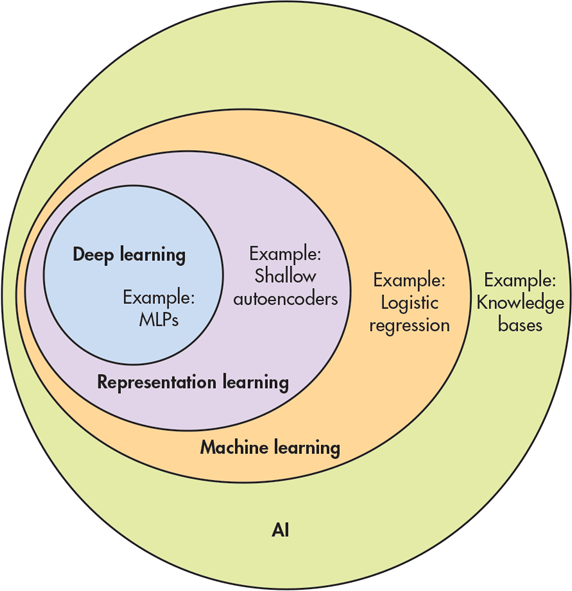
\includegraphics[width=0.6\textwidth]{fig/aiVennDiagram.png}
  \end{figure}
  \tiny
  \vspace{-1cm}
  \textit{[From \href{http://www.deeplearningbook.org/}{\color{blue}{MIT Press book Deep Learning}}]}
\end{frame}

\begin{frame}{1. Intro: Qu'est ce que le \textit{Machine Learning}}
  \begin{itemize}
  \item Les principaux types d'apprentissage:
  \end{itemize}
  \hspace{0.25\textwidth}
  \begin{beamerboxesrounded}[scheme=suppervise,width=0.5\textwidth]{\textcolor{black}{Supervisé}}
    \begin{itemize}
      \tiny
    \item Utilise des données \textit{labélisées}
    \item La machine apprend par l'exemple
    \item \textit{Prédis} le résultat pour de nouveaux événements
    \item Problèmes de régression et de classification
    \item Regression linéaire et logistique
    \item Réseaux de Neurones
    \item Arbres de décisions
    \end{itemize}
  \end{beamerboxesrounded}

  \vfill
  
  \begin{minipage}{.5\textwidth}
    \begin{beamerboxesrounded}[scheme=suppervise,width=0.95\textwidth]{\textcolor{black}{Non-supervisé}}
      \begin{itemize}
        \tiny
      \item Données non \textit{labélisées}
      \item La machine apprend par elle même à indentifier une structure
      \item Évaluation des performances compliqué.
      \item Problèmes de classification, réduction de dimensions
      \item K-means
      \item Analyse en Composante Principale
      \end{itemize}
    \end{beamerboxesrounded}
  \end{minipage}
  \hfill
  \begin{minipage}{.5\textwidth}
    \begin{beamerboxesrounded}[scheme=suppervise,width=0.95\textwidth]{\textcolor{black}{Par renforcement}}
      \vspace{0.5cm}
      \begin{itemize}
        \tiny
      \item Un agent A, effectue une action Ac, l'environnement E lui renvoie une récompense.
      \item Récompenses à court et long terme
      \item Utilisé par Deepmind (alphaGo)
      \end{itemize}
      \vspace{0.5cm}
    \end{beamerboxesrounded}
  \end{minipage}  
\end{frame}
